\documentclass{beamer}
\usetheme{Warsaw}
%Information to be included in the title page:

% using package
\usepackage{ graphicx }%插入圖片
\usepackage{ bbold } %characteristic function notation
\usepackage{ amssymb }
\usepackage{ braket }
\usepackage{bibentry} %citation
\usepackage{makecell}


%new commands
\newcommand{\notimplies}{%
  \mathrel{{\ooalign{\hidewidth$\not\phantom{=}$\hidewidth\cr$\implies$}}}}
\DeclareMathOperator*{\argmin}{arg\,min}
\DeclareMathOperator*{\argmax}{arg\,max}

\title[FT-report\hspace{2em}\insertframenumber/ \inserttotalframenumber]{Non-linear Constrained Optimization Problem using Byzantine Distributed Optimization Algorithm}
\subtitle{FT-report group 15}
\author{Ming-Yu Chung, Po-Yu Chen}
\institute{}
\date{December 2022}

\begin{document}
\frame{\titlepage}


%-------------------------------------------------------------------------------------------------------------------------
%Outline
\begin{frame}{Outline}
\begin{itemize}
\item \textbf{Introduction of Byzantine distributed optimization problem and our goal}
\item \textbf{Linearization method for constrained optimization problem}
\item \textbf{Proposed algorithm}
\end{itemize}
\end{frame}

%-----------------------------------------------------------------------------------------------------------------------------
%Introduction of Byzantine distributed optimization problem
\begin{frame}{Introduction of Byzantine distributed optimization problem}
    \centering
    \textbf{Introduction of Byzantine distributed optimization problem}
\end{frame}

\begin{frame}{Introduction of Byzantine distributed optimization problem}
\textbf{Byzantine distributed optimization problem} can be discribed as following setting:
\begin{enumerate}
    \item \textbf{Agent}: There are m agents. For $i$-th agent, he holds a cost function $C_i:\mathbb{R}^n \rightarrow \mathbb{R}$ and then send some information of $C_i(x)$ to the central server. We say the $i$-th agent is a Byzantine faulty agent if he send an incorrect information to central server. Otherwise, we call it is an honest agent.
    \item \textbf{Central server:} Central server aims to utilize the information from each agent to solve following optimization problem:
    \begin{align}
        \argmin_{x\in B} \sum_{i\in\mathcal{H}} C_i(x), \label{bdop}
    \end{align}
    where $B \subset \mathbb{R}^n$ is some compact set and $\mathcal{H}$ is the index set of honest agents.
\end{enumerate}
\end{frame}

\begin{frame}{Introduction of Byzantine distributed optimization problem}
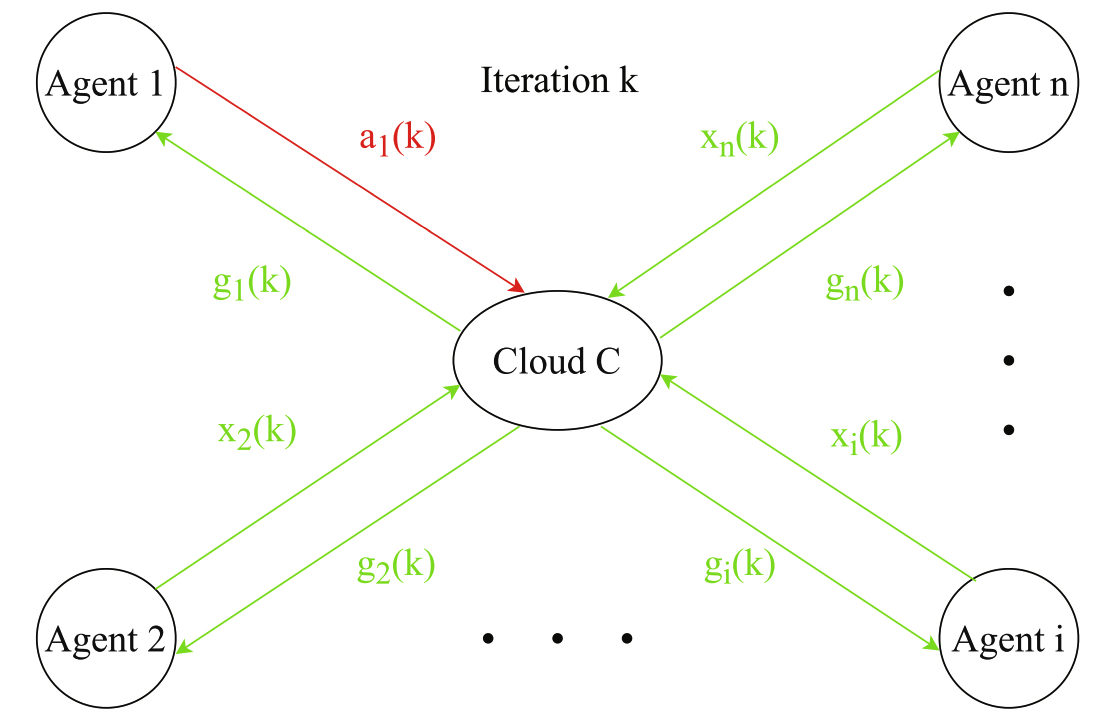
\includegraphics[scale=0.27]{fig/byzantine_fault.jpg} \cite {xu2022resilient} 
\end{frame}

\begin{frame}{Byzantine distributed optimization algorithm}
\cite{su2016fault, gupta2019byzantine1, gupta2019byzantine2, liu2021approximate} have shown that \alert{the exact fault tolerance problem (\ref{bdop}) cannot be solved} without some specific condition ($2f$-redundancy). Hence, in this project, we always assume $2f$-redundancy is satisfied. \newline

\textbf{Byzantine distributed optimization algorithm (BDOA)} is the algorithm to solve (\ref{bdop}). For example:

\begin{itemize}
    \item \textbf{Gradient-Filter-based Distributed Gradient Descent:} mitigates the detrimental impact of incorrect gradients
    \newline
    
     E.g., comparative gradient elimination (CGE) \cite {gupta2020byzantine3}, coordinate-wise trimmed mean (CWTM) \cite {su2016fault}, geometric median-of-means (GMoM) \cite {chen2017distributed}
\end{itemize}
    
\end{frame}

\begin{frame}{Our goal}
In this project, we consider the following constrained optimization problem:
$$
(P0)
\begin{cases}
    \argmin_{x\in B} &C_0(x)\\
    \text{subject to} &C_i(x) \leq 0, \text{ where } i \in [m].\label{P0}
\end{cases}
$$

We want to \alert{utilize the technique of (BDOA) to enhance the performance of some existing constrained optimization algorithm on (P0)}. To be more specific, we want to improve linearization method \cite{wilson2012linearization}.

\end{frame}

%--------------------------------------------------------------------------------------------------------------------------
%Linearization method
\begin{frame}{Linearization method}
    \centering
    \textbf{Linearization method}
\end{frame}

\begin{frame}{Linearization method}
At first, we approximate $(P0)$ as follows:
$$
(P1)
\begin{cases}
    \argmin_{p} &C_0(x) + \langle C'_0(x), p\rangle + \|p\|^2 \\
    \text{subject to} &C_i(x) + \langle C'_i(x), p\rangle \leq 0, \text{ where } i \in [m].\label{P1}
\end{cases}
$$
In \cite{wilson2012linearization}, we can solve $(P1)$ iteratively to obtain the solution of $(P0)$. To more specific, we consider following algorithm:
\begin{enumerate}
    \item Obtain direction $p^k$ by solving $(P1)$ at $x^k$.
    \item \alert{Approximate some suitable step size coefficient $\alpha^k > 0$}.
    \item Update $x^{k+1}\leftarrow x^k + \alpha^k \cdot p^k$.
    \item $k \leftarrow k+1$ and back to step 1.
\end{enumerate}
\alert{(Remark. If the linearization is terrible for some $C_i(x)$, the $\alpha^k$ will be very small and hence make the algorithm inefficient.)}
\end{frame}

%----------------------------------------------------------------------------------------------------
%Proposed method
\begin{frame}{Proposed Method}
\centering
\textbf{Proposed Method}
\end{frame}

\begin{frame}{Proposed method}
In this project, we aim develop an optimization algorithm to improve the performance of linearization method on (P0).
\newline

Here, we consider \alert{``linearization is terrible" as a fault} (i.e. $\alpha$ is too small) and apply \textbf{(BDOA)} on (P1). We can obtain the optimal point of 
$$
(PB)
\begin{cases}
    \argmin_{x\in B} &C_0(x)\\
    \text{subject to} &C_i(x) \leq 0, \text{ where } i \in \mathcal{H}.
\end{cases}
$$
\end{frame}

\begin{frame}{Proposed method}
 For the Byzantine faulty agents,
 $$
(PC)
\begin{cases}
    \argmin_{x\in B} &C_0(x)\\
    \text{subject to} &C_i(x) \leq 0, \text{ where } i \in \mathcal{B},
\end{cases}
$$
we utilize \textbf{central path method} and \textbf{proximal point method} \cite{boyd2004convex}.
\newline

Finally, in order to solve the original problem (P0). We utilize the \textbf{proximal gradient method} \cite{boyd2004convex} to hybrid (PB) and (PC). In short, we consider following algorithm:
\begin{enumerate}
    \item Update $x^k$ with \textbf{(BDOA)} and identify the byzantine faulty agents on (P0).
    \item Update $x^{k+1}$ with \textbf{central path method} and \textbf{proximal point method} on $(PC)$.
    \item $k\leftarrow k+2$ and back to step 1.
\end{enumerate}

(Some similar works : \cite{li2010hybrid, xu2022resilient})
\end{frame}

%-------------------------------------------------------------------------
%experiment
\begin{frame}{Experiment}
    \centering
    \textbf{Experiment}
\end{frame}

\begin{frame}{Experiment}
     The experiment has been conducted with three settings as Table~\ref{tab1} shown. The number of iterations is set as 20. We introduce a loss function to evaluate the optimization process:
     
    \begin{equation*}
        \text{Loss}(X) = f_{0}(X) + \sum_{i \in [m]} k_0 \cdot \text{ReLU}(C_{i}(X))
    \end{equation*}
    
    where $f_{0}$ is the objective function, $[m]$ is the index set of constraints, and $k_0$ - the "penalty" coefficient - is a hyper-parameter greater than zero. Here we set $k_0$ as 10000. Then we plot the loss values during the optimization process, as shown in Fig.~\ref{fig1}, Fig.~\ref{fig2} and Fig.~\ref{fig3}. Note that the values are the results of taken the logarithm.
\end{frame}

\begin{frame}{Experiment}
    \begin{table}[htbp]
        \centering
        \caption{Experiment settings}
        \scalebox{0.8}{    
            \begin{tabular}[]{cccc}
                \hline 
                Setting & Objective Function & Constraints & Initial Point ($X_{0}$) \\
                \hline 
                1 & $f(x, y) = y^{2} -3$ & \makecell{$10^{x} - 10^{-1} \leqslant 0$ \\ 
                $10^{y} - 10^{-3} \leqslant 0 $} & \makecell{$(3.0, -2.0)$ \\ $(-4.0, 9.0$)}  \\
                \hline 
                2 & $f(x, y) = y^{2} - 3$ & \makecell{$10^{x} - 10^{-1} \leqslant 0 $ \\ 
                $10^{y} - 10^{-3} \leqslant 0$ \\ $x^{2}+y^{2}-20 \leqslant 0$} & 
                \makecell {$(3.0, -2.0)$ \\ $(3.0, -20.0)$} \\
                \hline
                3 & $f(x, y) = x^{2} + y^{2} + 10$ & \makecell{$x^{6} + y^{6} - 20 \leqslant 0 $ \\
                $x^{2} + y^{2} - 10 \leqslant 0$ \\
                $y^{8} - 20 \leqslant 0 $ \\ $x+y-10 \leqslant 0$ \\ $3x-2y+1 \leqslant 0$} & 
                \makecell{$(30.0, -8.0)$ \\ $(-100.0, 5.0)$} \\
                \hline
            \end{tabular}
        }
        \label{tab1}
    \end{table}
\end{frame}

\begin{frame}{Experiment}
    \begin{figure}[htbp]
    \centerline{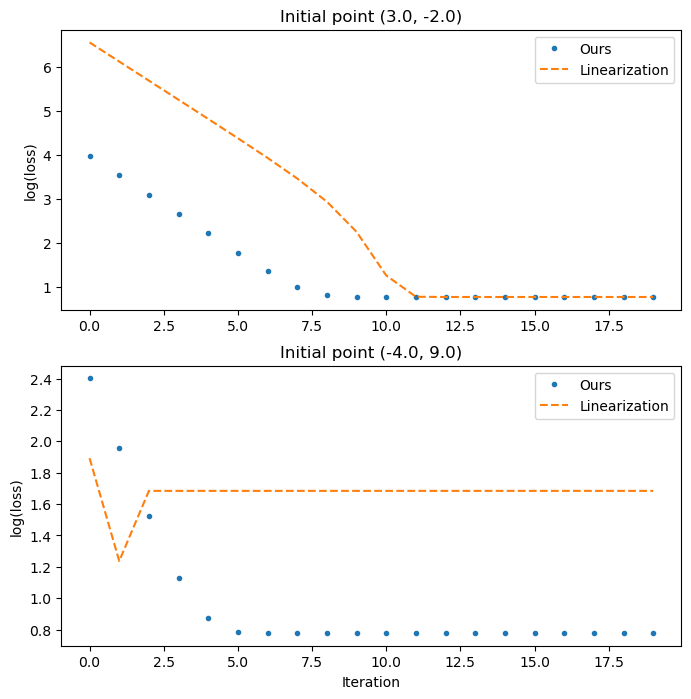
\includegraphics [scale=0.3]{./fig/setting1.png}}
    \caption{Experiment result of setting 1.}
    \label{fig1}
    \end{figure}
\end{frame}

\begin{frame}{Experiment}
    \begin{figure}[htbp]
    \centerline{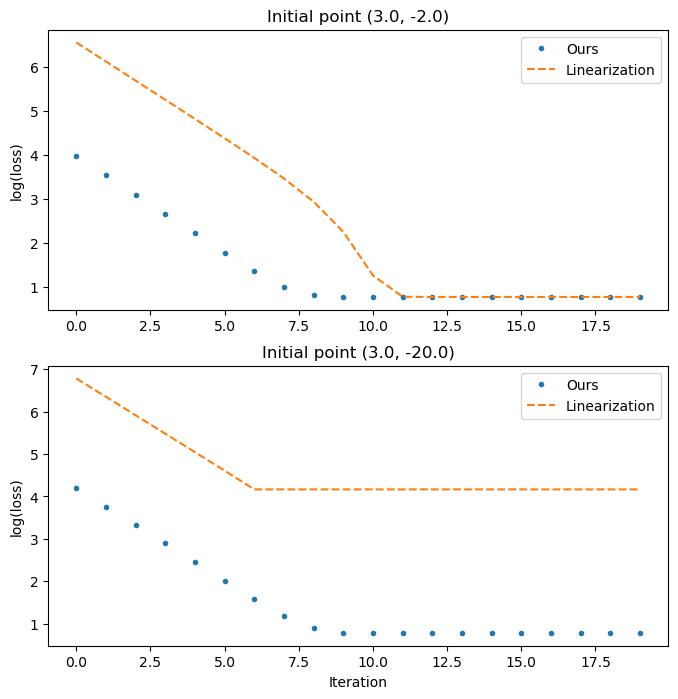
\includegraphics [scale=0.3]{./fig/setting2.png}}
    \caption{Experiment result of setting 2.}
    \label{fig2}
    \end{figure}
\end{frame}

\begin{frame}{Experiment}
    \begin{figure}[htbp]
    \centerline{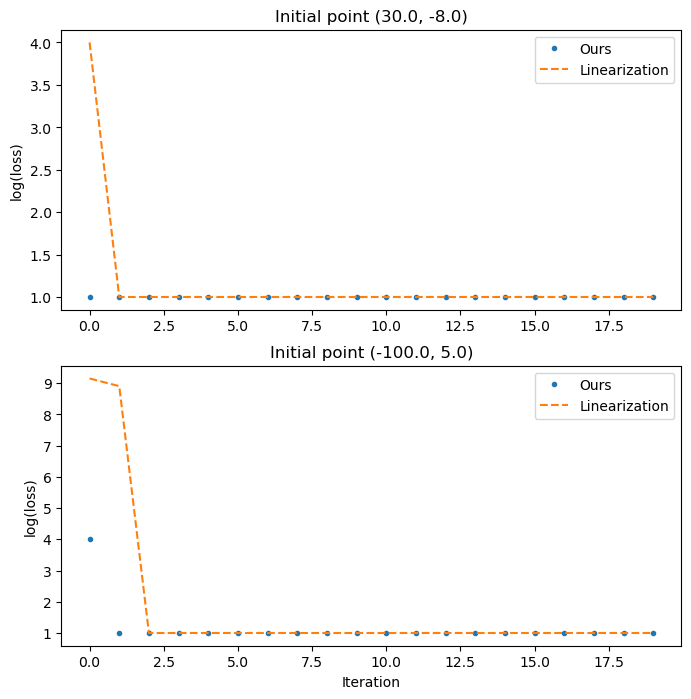
\includegraphics [scale=0.3]{./fig/setting3.png}}
    \caption{Experiment result of setting 3.}
    \label{fig3}
    \end{figure}
\end{frame}

%--------------------------------------------------------------------------
%Conclusion
\begin{frame}{Conclusion}
    \centering
    \textbf{Conclusion}
\end{frame}
\begin{frame}{Conclusion}
\begin{enumerate}
    \item We proposed an algorithm based on BDOA and linearization method for non-linear constrained optimization problems.
    \item The experimental results show that our algorithm is experimentally better than linearization method.
\end{enumerate}
\end{frame}

%--------------------------------------------------------------------------
%Future works
\begin{frame}{Future works}
    \centering
    \textbf{Future works}
\end{frame}
\begin{frame}{Future works}
    \begin{enumerate}
    \item Provide theoretical proof to show our algorithm is better than linearization method,  when the optimization problem which we consider is sufficiently unsuitable for linear approximation.
    \item Provide an estimation of hyper-parameters.
    \item Do more experiments to show the feasibility of our algorithm.
    \end{enumerate}
\end{frame}

%--------------------------------------------------------------------------
\begin{frame}{Thanks}
    \centering
    \textbf{Thanks for listening}
\end{frame}
%--------------------------------------------------------------------------------------------------------------------------
%References
\begin{frame}[allowframebreaks]{References}
    \bibliographystyle{amsalpha}
    \bibliography{ref}
\end{frame}

\end{document}






